% questions.tex —— 2008 年·普通高等学校招生考试·辽宁卷·理科 · 题目内容片段（无答案）
% 由 tools/generate_projects.py 依来源总账自 2008/2008_数学真题_辽宁理_试题.md 生成，勿手改（改源 MD 后重跑）


\gkpart{一、选择题}

\begin{question}
\gkti{1}已知集合 $M=\left\{x\mid \dfrac{x+3}{x-1}<0\right\}$，$N=\{x\mid x\leqslant-3\}$，则集合 $\{x\mid x\geqslant1\}=$（　）

（A）$M\cap N$

（B）$M\cup N$

（C）$\complement_{\mathbf R}(M\cap N)$

（D）$\complement_{\mathbf R}(M\cup N)$

\end{question}
\begin{question}
\gkti{2}$\lim\limits_{n\to\infty}\dfrac{1+3+5+\cdots+(2n-1)}{n(2n+1)}=$（　）

（A）$\dfrac14$

（B）$\dfrac12$

（C）$1$

（D）$2$

\end{question}
\begin{question}
\gkti{3}圆 $x^2+y^2=1$ 与直线 $y=kx+2$ 没有公共点的充要条件是（　）

（A）$k\in(-\sqrt2,\sqrt2)$

（B）$k\in(-\infty,-\sqrt2)\cup(\sqrt2,+\infty)$

（C）$k\in(-\sqrt3,\sqrt3)$

（D）$k\in(-\infty,-\sqrt3)\cup(\sqrt3,+\infty)$

\end{question}
\begin{question}
\gkti{4}复数 $\dfrac1{-2+\mathrm i}+\dfrac1{1-2\mathrm i}$ 的虚部是（　）

（A）$\dfrac15\mathrm i$

（B）$\dfrac15$

（C）$-\dfrac15\mathrm i$

（D）$-\dfrac15$

\end{question}
\begin{question}
\gkti{5}已知 $O$，$A$，$B$ 是平面上的三个点，直线 $AB$ 上有一点 $C$，满足 $2\overrightarrow{AC}+\overrightarrow{CB}=\boldsymbol 0$，则 $\overrightarrow{OC}=$（　）

（A）$2\overrightarrow{OA}-\overrightarrow{OB}$

（B）$-\overrightarrow{OA}+2\overrightarrow{OB}$

（C）$\dfrac23\overrightarrow{OA}-\dfrac13\overrightarrow{OB}$

（D）$-\dfrac13\overrightarrow{OA}+\dfrac23\overrightarrow{OB}$

\end{question}
\begin{question}
\gkti{6}设 $P$ 为曲线 $C:y=x^2+2x+3$ 上的点，且曲线 $C$ 在点 $P$ 处切线倾斜角的取值范围是 $\left[0,\dfrac{\pi}{4}\right]$，则点 $P$ 横坐标的取值范围是（　）

（A）$\left[-1,-\dfrac12\right]$

（B）$[-1,0]$

（C）$[0,1]$

（D）$\left[\dfrac12,1\right]$

\end{question}
\begin{question}
\gkti{7}$4$ 张卡片上分别写有数字 $1$，$2$，$3$，$4$，从这 $4$ 张卡片中随机抽取 $2$ 张，则取出的 $2$ 张卡片上的数字之和为奇数的概率为（　）

（A）$\dfrac13$

（B）$\dfrac12$

（C）$\dfrac23$

（D）$\dfrac34$

\end{question}
\begin{question}
\gkti{8}将函数 $y=2^x+1$ 的图象按向量 $\boldsymbol a$ 平移得到函数 $y=2^{x+1}$ 的图象，则（　）

（A）$\boldsymbol a=(-1,-1)$

（B）$\boldsymbol a=(1,-1)$

（C）$\boldsymbol a=(1,1)$

（D）$\boldsymbol a=(-1,1)$

\end{question}
\begin{question}
\gkti{9}一生产过程有 $4$ 道工序，每道工序需要安排一人照看。现从甲、乙、丙等 $6$ 名工人中安排 $4$ 人分别照看一道工序，第一道工序只能从甲、乙两工人中安排 $1$ 人，第四道工序只能从甲、丙两工人中安排 $1$ 人，则不同的安排方案共有（　）

（A）$24$ 种

（B）$36$ 种

（C）$48$ 种

（D）$72$ 种

\end{question}
\begin{question}
\gkti{10}已知点 $P$ 是抛物线 $y^2=2x$ 上的一个动点，则点 $P$ 到点 $(0,2)$ 的距离与 $P$ 到该抛物线准线的距离之和的最小值为（　）

（A）$\dfrac{\sqrt{17}}{2}$

（B）$3$

（C）$\sqrt5$

（D）$\dfrac92$

\end{question}
\begin{question}
\gkti{11}在正方体 $ABCD-A_1B_1C_1D_1$ 中，$E$，$F$ 分别为棱 $AA_1$，$CC_1$ 的中点，则在空间中与三条直线 $A_1D_1$，$EF$，$CD$ 都相交的直线（　）

（A）不存在

（B）有且只有两条

（C）有且只有三条

（D）有无数条

\end{question}
\begin{question}
\gkti{12}设 $f(x)$ 是连续的偶函数，且当 $x>0$ 时 $f(x)$ 是单调函数，则满足 $f(x)=f\left(\dfrac{x+3}{x+4}\right)$ 的所有 $x$ 之和为（　）

（A）$-3$

（B）$3$

（C）$-8$

（D）$8$

\end{question}
\gkpart{二、填空题}

\begin{question}
\gkti{13}函数 $y=\begin{cases}x+1,&x<0,\\ \mathrm e^x,&x\geqslant0,\end{cases}$ 的反函数是\gkblank{}。

\end{question}
\begin{question}
\gkti{14}在体积为 $4\sqrt3\pi$ 的球的表面上有 $A$，$B$，$C$ 三点，$AB=1$，$BC=\sqrt2$，$A$，$C$ 两点的球面距离为 $\dfrac{\sqrt3}{3}\pi$，则球心到平面 $ABC$ 的距离为\gkblank{}。

\end{question}
\begin{question}
\gkti{15}已知 $\left(1+x+x^2\right)\left(x+\dfrac1{x^3}\right)^n$ 的展开式中没有常数项，$n\in\mathbf N^*$ 且 $2\leqslant n\leqslant8$，则 $n=$\gkblank{}。

\end{question}
\begin{question}
\gkti{16}已知 $f(x)=\sin\left(\omega x+\dfrac{\pi}{3}\right)$（$\omega>0$），$f\left(\dfrac{\pi}{6}\right)=f\left(\dfrac{\pi}{3}\right)$，且 $f(x)$ 在区间 $\left(\dfrac{\pi}{6},\dfrac{\pi}{3}\right)$ 有最小值，无最大值，则 $\omega=$\gkblank{}。

\end{question}
\gkpart{三、解答题}

\begin{question}
\gkti{17}在 $\triangle ABC$ 中，内角 $A$，$B$，$C$ 对边的边长分别是 $a$，$b$，$c$。已知 $c=2$，$C=\dfrac{\pi}{3}$。

（1）若 $\triangle ABC$ 的面积等于 $\sqrt3$，求 $a$，$b$；

（2）若 $\sin C+\sin(B-A)=2\sin2A$，求 $\triangle ABC$ 的面积。

\end{question}
\begin{question}
\gkti{18}某批发市场对某种商品的周销售量（单位：吨）进行统计，最近 $100$ 周的统计结果如下表所示：

\begin{center}
\begin{tabular}{llll}
\toprule
周销售量 & $2$ & $3$ & $4$ \\
\midrule
频数 & $20$ & $50$ & $30$ \\
\bottomrule
\end{tabular}
\end{center}

（1）根据上面统计结果，求周销售量分别为 $2$ 吨、$3$ 吨和 $4$ 吨的频率；

（2）已知每吨该商品的销售利润为 $2$ 千元，$\xi$ 表示该种商品两周销售利润的和（单位：千元）。若以上述频率作为概率，且各周的销售量相互独立，求 $\xi$ 的分布列和数学期望。

\Needspace{0.4\textheight}
\end{question}
\begin{question}
\gkti{19}如图，在棱长为 $1$ 的正方体 $ABCD-A'B'C'D'$ 中，$AP=BQ=b$（$0<b<1$），截面 $PQEF\parallel A'D$，截面 $PQGH\parallel AD'$。

（1）证明：平面 $PQEF$ 和平面 $PQGH$ 互相垂直；

（2）证明：截面 $PQEF$ 和截面 $PQGH$ 面积之和是定值，并求出这个值；

（3）若 $D'E$ 与平面 $PQEF$ 所成的角为 $45^\circ$，求 $D'E$ 与平面 $PQGH$ 所成角的正弦值。
\nopagebreak[4]
\begin{center}% 2008 年辽宁卷理科第 19 题：棱长 1 的正方体 ABCD-A'B'C'D'，AP=BQ=b，
%   截面 PQEF∥A'D，截面 PQGH∥AD'。
% 来源 PDF：gaokaomath-src/普通高考/2008/2008辽宁理.pdf
% SHA-256：1de96dd843dfb46e9b6e94b1e78277acebbbbb004eb3350c7d1820702b25f2d2
% 原页：2008辽宁理.pdf 第 1 页（A3 三栏）第 3 栏，书页码 463。
% 重绘依据：与文科卷第 19 题同一几何体同构图（理科第 (3) 问条件不同，图形一致）。
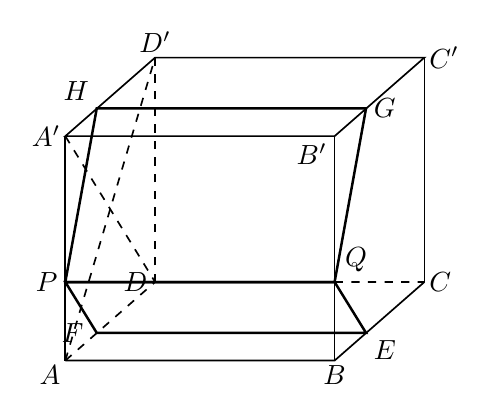
\begin{tikzpicture}[scale=0.95, semithick, every node/.style={inner sep=1.5pt}]
  \coordinate (A) at (0.00,0.00);
  \coordinate (B) at (3.60,0.00);
  \coordinate (C) at (4.80,1.05);
  \coordinate (D) at (1.20,1.05);
  \coordinate (A1) at (0.00,3.00);
  \coordinate (B1) at (3.60,3.00);
  \coordinate (C1) at (4.80,4.05);
  \coordinate (D1) at (1.20,4.05);

  \coordinate (P) at (0.00,1.05);
  \coordinate (Q) at (3.60,1.05);
  \coordinate (E) at (4.02,0.37);
  \coordinate (F) at (0.42,0.37);
  \coordinate (G) at (4.02,3.37);
  \coordinate (H) at (0.42,3.37);

  % 立方体可见棱
  \draw (A) -- (B) -- (C);
  \draw (A) -- (A1);
  \draw (B) -- (B1);
  \draw (C) -- (C1);
  \draw (A1) -- (B1) -- (C1) -- (D1) -- cycle;

  % 隐藏棱
  \draw[dashed] (A) -- (D) -- (C);
  \draw[dashed] (D) -- (D1);

  % 两个截面
  \draw[line width=0.9pt] (P) -- (Q) -- (E) -- (F) -- cycle;
  \draw[line width=0.9pt] (P) -- (Q) -- (G) -- (H) -- cycle;

  % 与截面平行的两条对角线
  \draw[dashed] (A1) -- (D);
  \draw[dashed] (A) -- (D1);

  \node[below left] at (A) {$A$};
  \node[below] at (B) {$B$};
  \node[right] at (C) {$C$};
  \node[left=1pt] at (D) {$D$};
  \node[left] at (A1) {$A'$};
  \node[below left=1pt] at (B1) {$B'$};
  \node[right] at (C1) {$C'$};
  \node[above] at (D1) {$D'$};
  \node[left=1pt] at (P) {$P$};
  \node[above right=2pt] at (Q) {$Q$};
  \node[below right=1pt] at (E) {$E$};
  \node[left=3pt] at (F) {$F$};
  \node[right=1pt] at (G) {$G$};
  \node[above left=1pt] at (H) {$H$};
\end{tikzpicture}
\end{center}
\nopagebreak[4]
\end{question}
\begin{question}
\gkti{20}在直角坐标系 $xOy$ 中，点 $P$ 到两点 $(0,-\sqrt3)$，$(0,\sqrt3)$ 的距离之和为 $4$，设点 $P$ 的轨迹为 $C$，直线 $y=kx+1$ 与 $C$ 交于 $A$，$B$ 两点。

（1）写出 $C$ 的方程；

（2）若 $\overrightarrow{OA}\perp\overrightarrow{OB}$，求 $k$ 的值；

（3）若点 $A$ 在第一象限，证明：当 $k>0$ 时，恒有 $\left|\overrightarrow{OA}\right|>\left|\overrightarrow{OB}\right|$。

\end{question}
\begin{question}
\gkti{21}在数列 $\{a_n\}$，$\{b_n\}$ 中，$a_1=2$，$b_1=4$，且 $a_n$，$b_n$，$a_{n+1}$ 成等差数列，$b_n$，$a_{n+1}$，$b_{n+1}$ 成等比数列。

（1）求 $a_2$，$a_3$，$a_4$ 及 $b_2$，$b_3$，$b_4$，由此猜测 $\{a_n\}$，$\{b_n\}$ 的通项公式，并证明你的结论；

（2）证明：$\dfrac1{a_1+b_1}+\dfrac1{a_2+b_2}+\cdots+\dfrac1{a_n+b_n}<\dfrac5{12}$。

\end{question}
\begin{question}
\gkti{22}设函数 $f(x)=\dfrac{\ln x}{1+x}-\ln x+\ln(x+1)$。

（1）求 $f(x)$ 的单调区间和极值；

（2）是否存在实数 $a$，使得关于 $x$ 的不等式 $f(x)\geqslant a$ 的解集为 $(0,+\infty)$？若存在，求 $a$ 的取值范围；若不存在，试说明理由。

\end{question}